\documentclass[type=dr, dr=rernat, accentcolor=tud7b,colorbacktitle, bigchapter, openright, twoside, 12pt ]{tudthesis}
\usepackage[english]{babel} 
\usepackage[utf8]{inputenc}
\usepackage{graphicx}
\usepackage{pstricks}
\usepackage{psfrag}
\usepackage{enumerate}
\usepackage{float}
\usepackage{epsfig}
%\usepackage{geometry}
\usepackage{subfigure}
\usepackage{rotating}
\usepackage{minitoc}
\usepackage{appendix}

%%%% 1 1/2 facher Zeilenabstand:	
\usepackage{setspace}
\onehalfspacing


\begin{document}
\thesistitle{Robust motion mitigation for (noncancerous) lesions in scanned ion beam therapy}{Robuste Methoden zur Verminderung der bewegunginduzierten Effekte f\"ur (nicht 
kanzer\"ose) L\"asionen in der Therapie mit nachgef\"uhrten Ionenstrahlen}
\author{MSc Anna Maria Constantinescu}
\birthplace{Bukarest, Rum\"anien}
\date{\today}
\referee{Prof. Dr. Marco Durante}{Dr. Christoph Bert}
\department{Fachbereich Physik}
\group{Prof. Durante\newline Institut f\"ur Festk\"orperphysik}
\dateofexam{}{}
\makethesistitle


\affidavit{Anna Constantinescu}

% \dominitoc
\tableofcontents

\chapter{Introduction}


\newpage

\section{Atrial fibrillation}

Atrial fibrillation (AF) is the most common caridac arrhthmia. It occurs in $\sim$2 \% of the general population leading to over six million patients in Europe \cite{ESC10} and over two million patients in the United States \cite{CE09}. The lifetime risk of developing AF is $\sim$ 25\% in people over forty. Since age is an important risk factor for this cardiac arrhymia the prevalence is estimated to double in the next fifty years due to the overall ageing of society.\newline

\begin{figure}[H]
\begin{center}
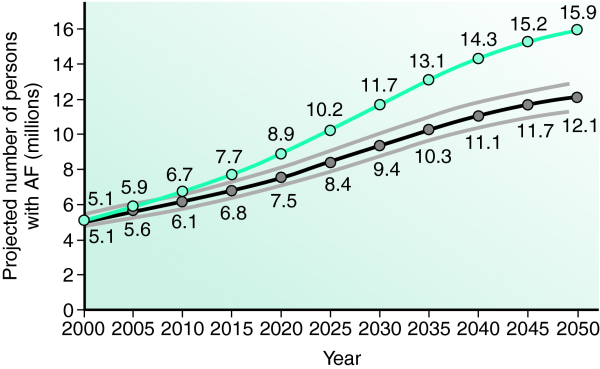
\includegraphics[scale=3]{af_incidences_us.png}
\caption{Trend of AF incidences. The black curve indicates the projected number of patients assuming no further increase in age-adjusted AF incidences. The green curve represents the trend assuming a continous increase in incident rates as evident in 1980 to 2000. Figure taken from \cite{Miy06}}
\label{USincidences}
\end{center}
\end{figure}

Even though not in itself life threatening, it dramatically alters the quality of life of the patients and drastically increases the risk of suffering a stroke. It is estimated that the stroke risk in AF patients is 5-fold. Moreover AF often remains undiagnosed (silent AF) and it is stated that one out of five acute strokes is attributed to AF \cite{ESC10}. Other late effects and related events include cognitive dysfuntions like vascular dementia and impairment of the left ventricular function. In general death rates are stated to double by AF \cite{ESC10}.\newline



\subsection*{Heart's conduction system}

The conduction system of the heart controls the generation and propagation of electrical signals, so called action potentials, that cause the heart muscle to contract and hence to pump blood \cite{Med}. The action potentials can originate spontaenously in any of the specialised cardiac muscle cells which form the conduction system. In a healthy heart each beat begins in the right atrium with an action potential from the sinoatrial (SA) node (see fig. \ref{condsys}). The SA node differs from the rest of the cardiac muscle cells by exhibiting a larger number of calcium channels. Depolarization is hence reached faster, shortening the intervals between different action potentials. This makes the SA node the natural pacemaker of the heart.
The signal then spreads across both atria causing the muscle cells to depolarize and hence to contract, a phase called the atrial systole which is represented as the P-wave in an ECG (see fig. \ref{ecg}). It is followed by a period of conduction (PR-segment in ECG) in which the signal enters the ventricels via the atrioventricular (AV) node. The AV node is located at the lower portion of the right atrium and is the passing point where every signal from the atria is received and slowly propagated to the ventricles. The action potentials pass the ventricles 
by entering the Bundle of His, spreading through the bundle brances and the Purkinje fibers and further along the ventricle walls. As the signal spreads the ventricles contract very rapidely and this ventricular systole is displayed in the QRS-complex in an ECG. Atrial repolarisation also occurs at this time, but any atrial activity is hidden in the ECG by the QRS complex. As the signal passes out of the ventricles, the ventricular walls start to relax (ventricular diastole). The T-wave marks this ventricular repolarisation. The sequence of these events and the corresponding ECG traces repeat with every single heartbeat.\newline

\vspace{-7cm}
\begin{figure}[H]
\begin{center}
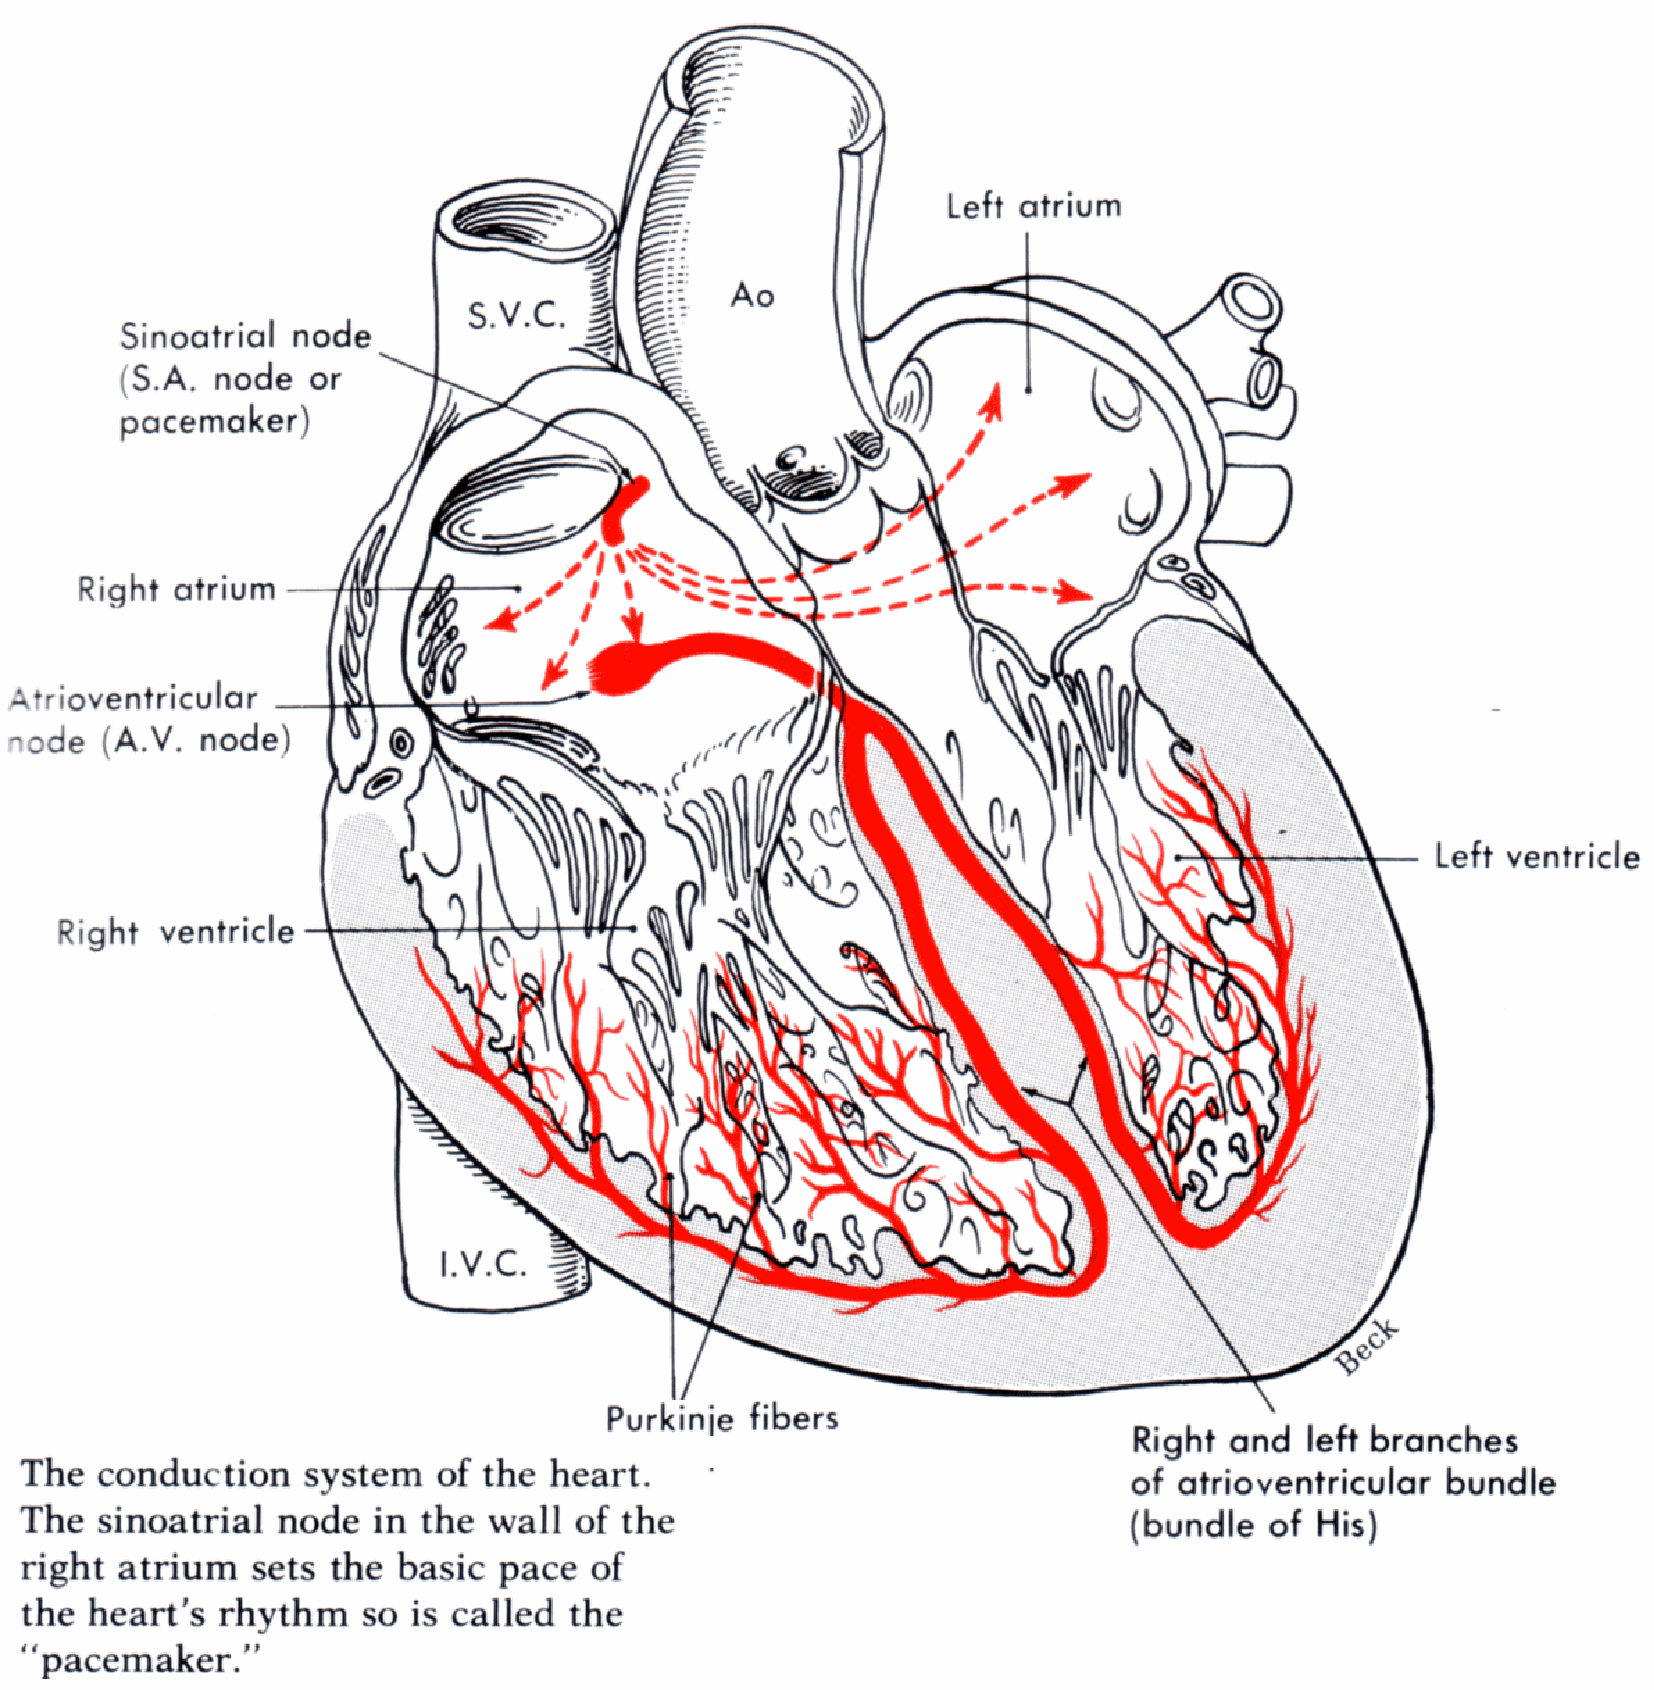
\includegraphics[scale=0.3]{conduction_system.png}
\caption{Scheme of the conduction system of the heart. Figure taken from \cite{amc}}
\label{condsys}
\end{center}
\end{figure}

\begin{figure}[H]
\begin{center}
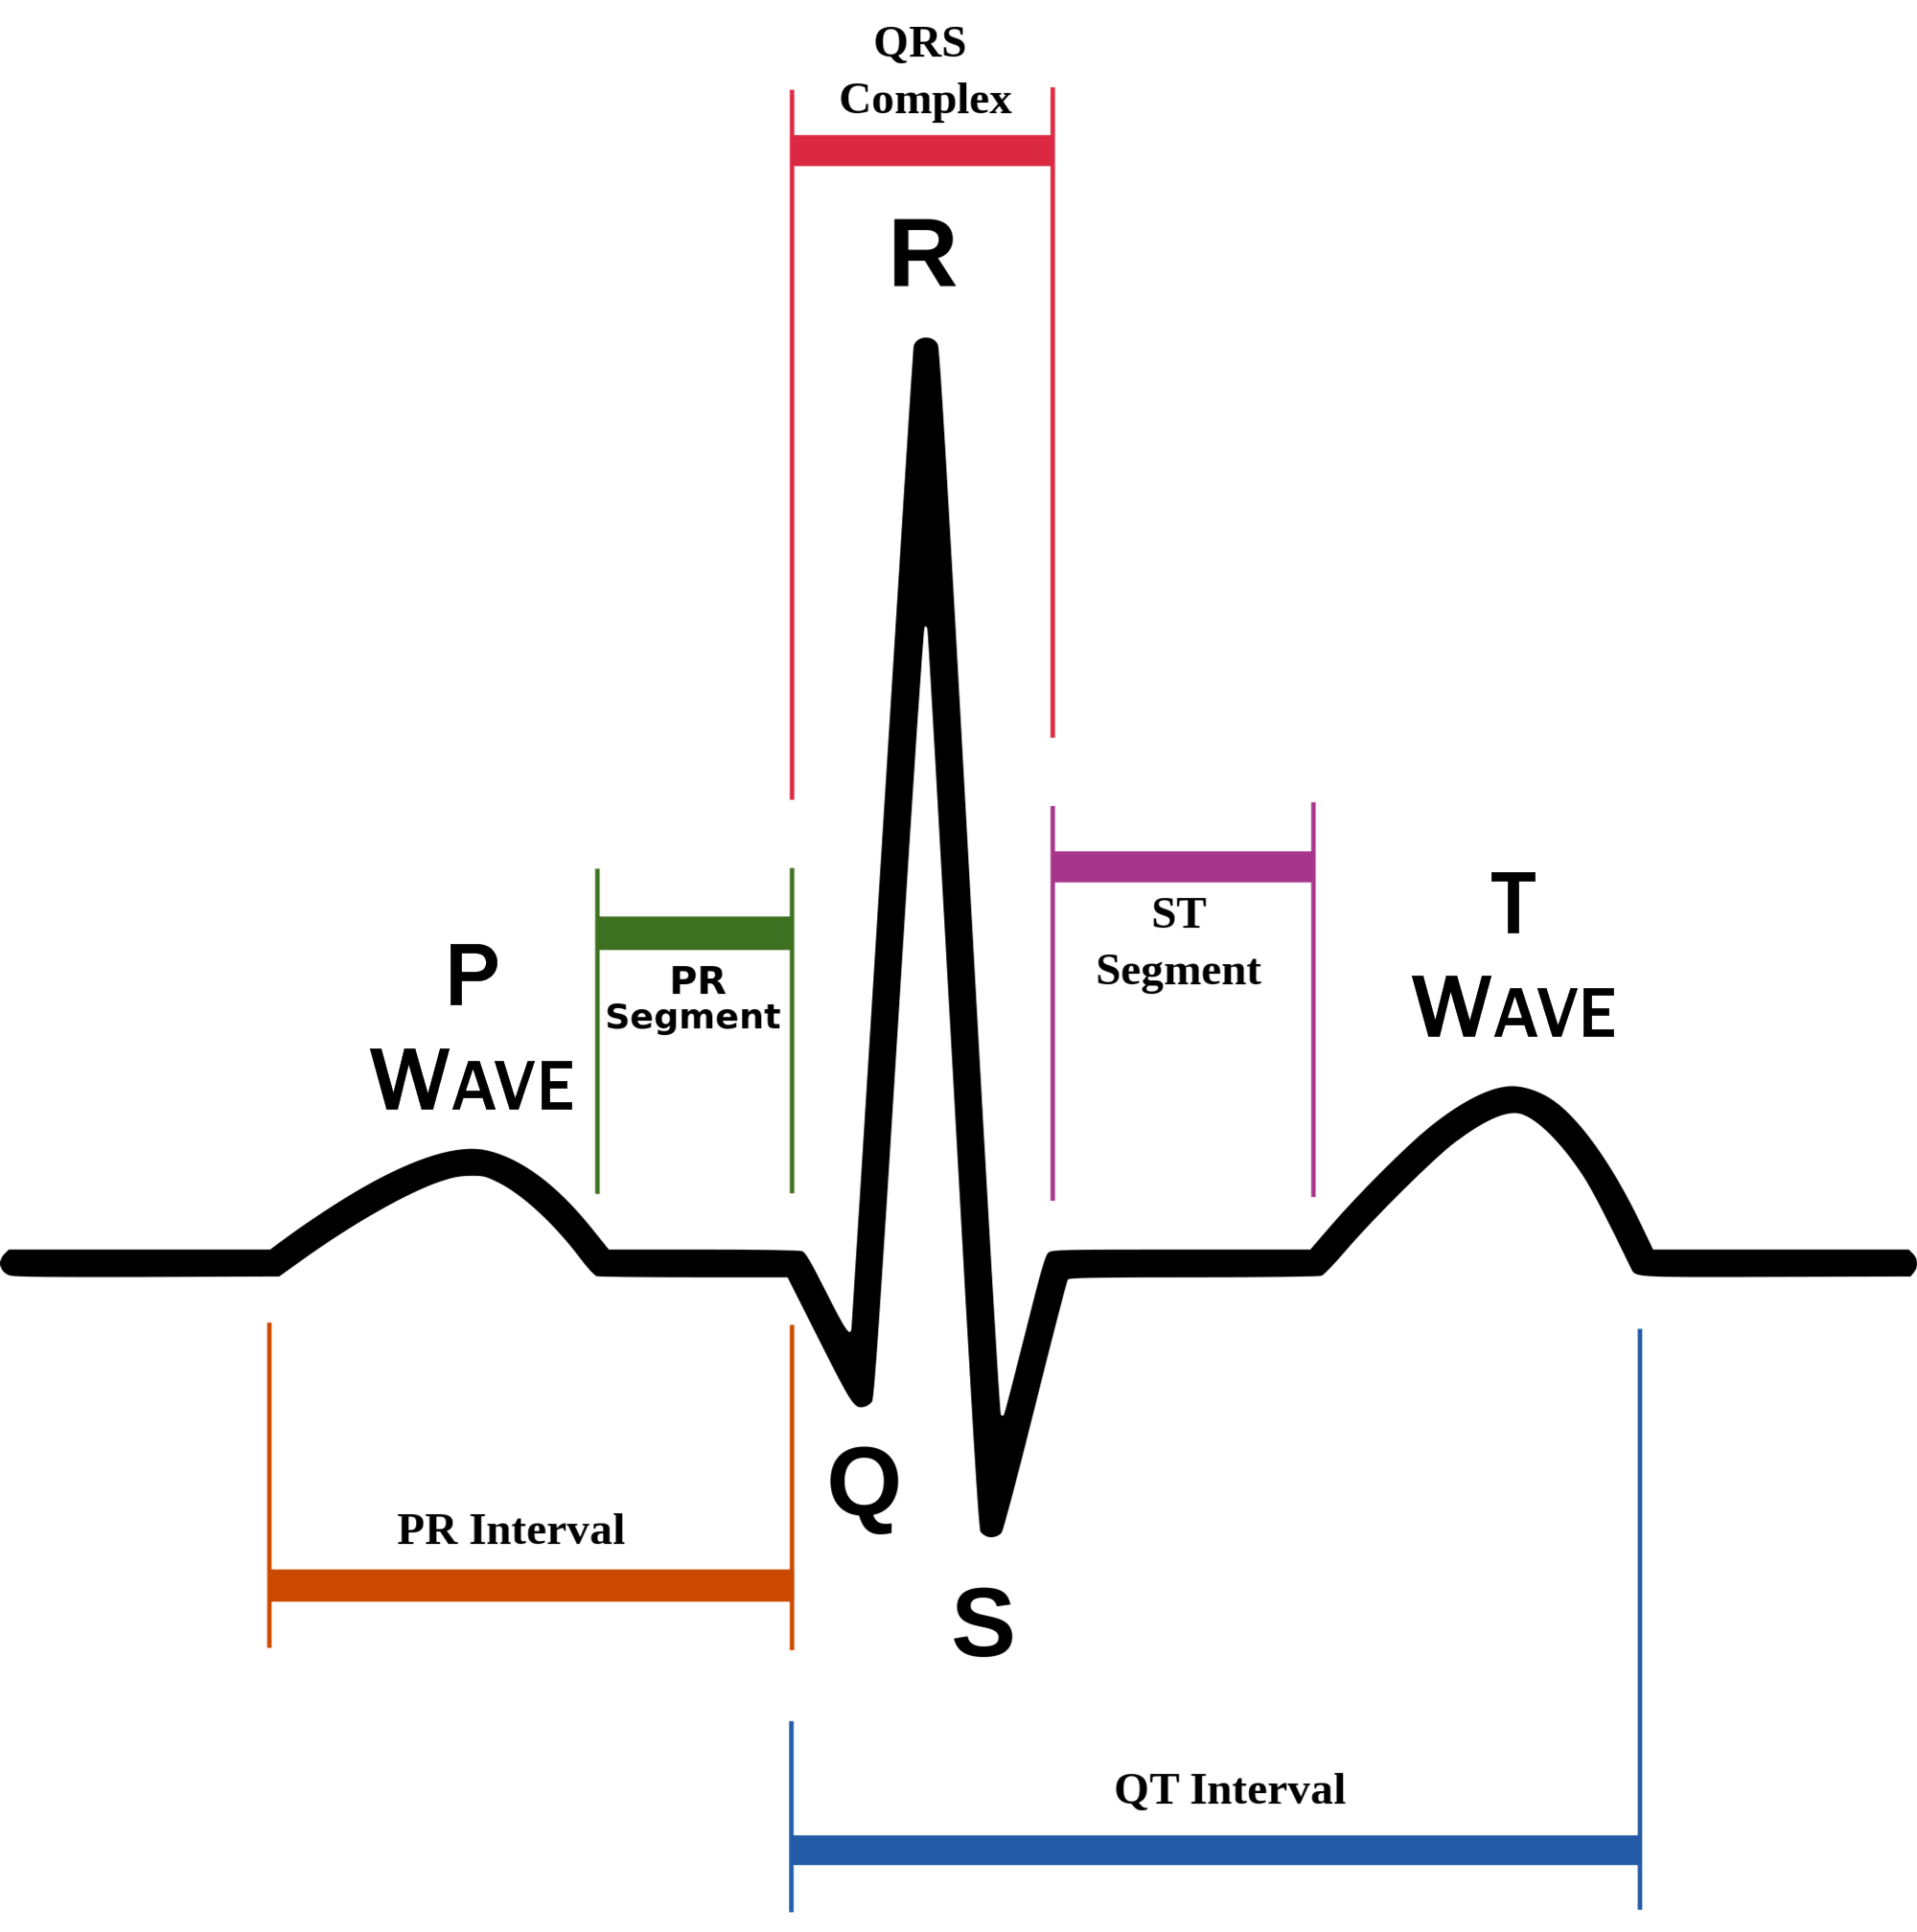
\includegraphics[scale=0.13]{ecg.png}
\caption{ECG trace of a normal heart beat. Figure taken from \cite{afib}}
\label{ecg}
\end{center}
\end{figure}

In AF the atria is fulfilling a quivering motion and is hence not able to sustain a healthy pumping rhythm. An examplary ECG trace for AF can be seen in figure \ref{af_ecg}
This is not in itself life threatening but it can dramatically alter the quality of life and drastically increases the risk of the patient of suffering a stroke. Possible reasons for this abnormal electrophysiology are stated in the next sections.

\begin{figure}[H]
\begin{center}
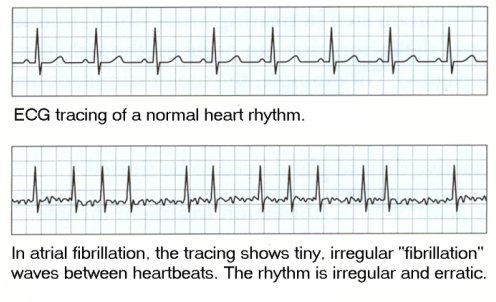
\includegraphics[scale=3]{AF_ECG.png}
\caption{ECG traces for a normal sinus rhythm (upper row) and for an AF patient (lower row). Figure taken from \cite{afib}}
\label{af_ecg}
\end{center}
\end{figure}

\newpage
\subsection*{Types of AF}

Based on the duration and presentation of the condition five types of AF are clinically distinguished \cite{ESC10} \cite{CE09}.

\begin{itemize} 
 \item[] \textbf{First diagnosed AF}: Valid for every patient presenting with AF for the first time. This classification independent of the duration, presence or severity of the condition. An episode must last for 30 seconds or longer to be considered a clinical AF.
 \item[] \textbf{Paroxysmal AF}: Recurrent episodes (two or more) of AF which is self-terminating within 48 hours. After this timespan the likelihood of spontaneous conversion is low.
 \item[] \textbf{Persistent AF}: Conditions which are present for longer than 7 days or which require cardioversion independent of the duration of the episode. 
 \item[] \textbf{Long-standing persistent AF}: continous episodes of persistent AF present for more than 1 year. Rhythm control interventions  are carried out in this patient group. 
 \item[] \textbf{Permanent AF}: classification when the existence of AF is accepted by patient and physician. Restoration and maintenance of sinus rhythm has either failed or has not been attempted. By definition rhythm control interventions are not carried out in these patient class.  
\end{itemize}

Furthermore \textbf{silent AF} may present as any form of the stated AF types. As the name indicates, the condition is asymptomatic and hence undiagnosed. It usually manifests as an AF related complication like an ischaemic stroke. About one third of people with AF are estimated to be unaware of their condition \cite{ESC10}.

\begin{figure}[H]
\begin{center}
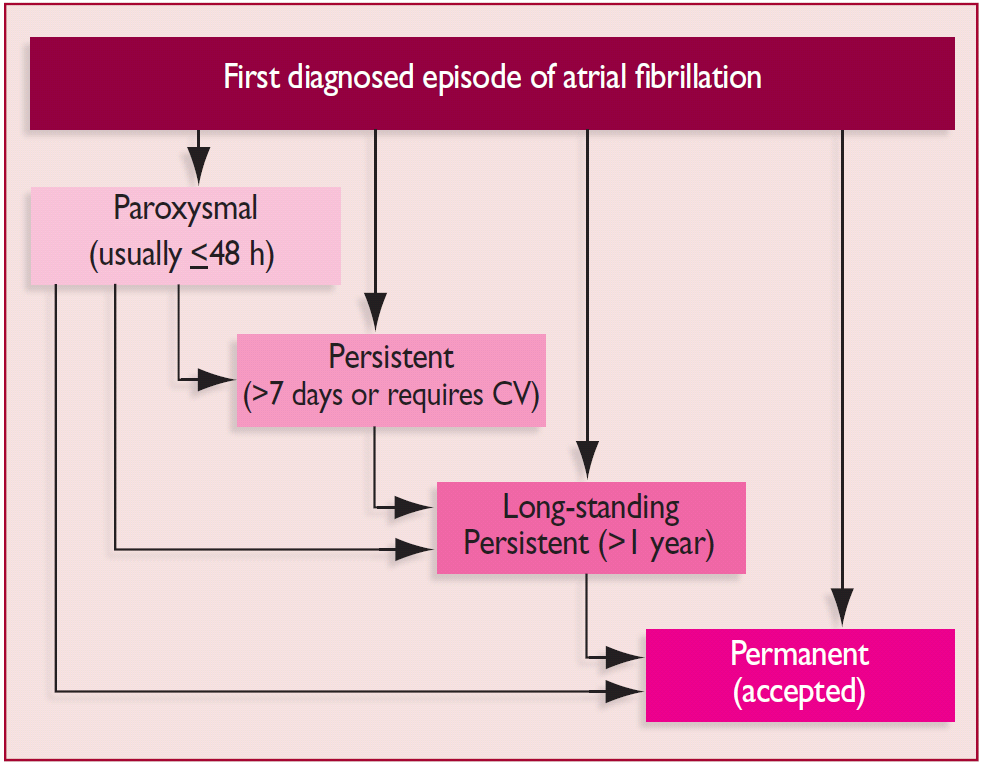
\includegraphics[scale=0.25]{af_types.png}
\caption{Different types of AF. Figure taken from \cite{ESC10}}
\label{ecg}
\end{center}
\end{figure}

Usually AF progresses over time. Starting as short and rare episodes the condition develops into longer and more frequent attacks \cite{ESC10}. 

\begin{figure}[H]
\begin{center}
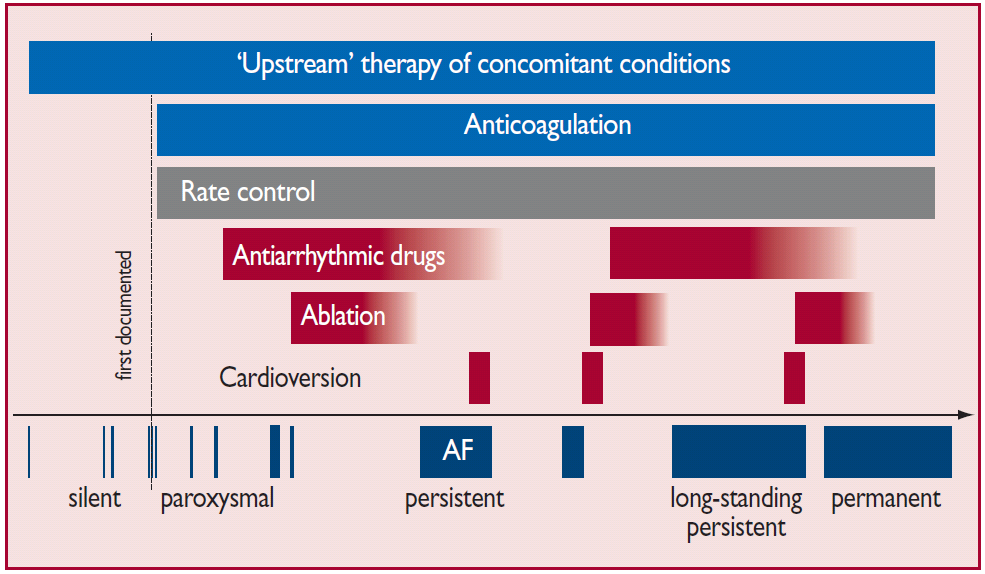
\includegraphics[scale=0.3]{af_over_time.png}
\caption{Typical time course of AF. The dark blue boxes show the different periods of AF. The upper bars indicate possible treatment possibilities at the different stages of AF. The light blue boxes represent medication uptake which should prevent the formation of blood clots. These medications are recommanded in the majority of AF patients. The red boxes indicate system relief therapies while the grey boxes represent rate control measures. Figure taken from \cite{ESC10}}
\label{afovertime}
\end{center}
\end{figure}



\subsection*{Possible causes for AF and risk factors}

The mechanisms of AF are multifactorial and not yet fully understood. The mechanisms may influence and sustain each other. Triggers for the initiation and perpetuation as well as a substrate for the maintenance are needed. Current research indiactes that one can distinguishes between focal mechanisms and multiple wavelets \cite{CE09}. For most patients with paroxysmal AF a localized, focal trigger can be identified such attempts are not successful in patients with persistent or permanent AF, where the multiple wavelet hypothesis is believed to be more accurate.\newline

An identified focal trigger site are the \textbf{pulmonary veins} (PVs). In a benchmark paper Ha\"{\i}ssagurre et al. \cite{Hai98} studied 45 patients with frequent episodes of AF ( 344 $\pm$ 326 minutes episodes per 24 hours) finding etopic beats \footnote{beats which arise from cells outside the region in the heart muscle ordinarily responsible for impulse formation} originating from the pulmonary veins in 94 \% of the cases. The underlying mechanism by which PVs become arrhythmogenic in some patients while it remains dormant in others is still not clear \cite{CE09}. The reason why PVs can become arrhythmogenic at all is based on stages during the embryonic development, in which the commom PV is incorporated into the left atrium. Immunohistochemical studies have shown that the composition of the PV and the smooth-walled portion of the left atrium are identical \cite{CE09} \cite{Dou06}. 

\begin{figure}[H]
\begin{center}
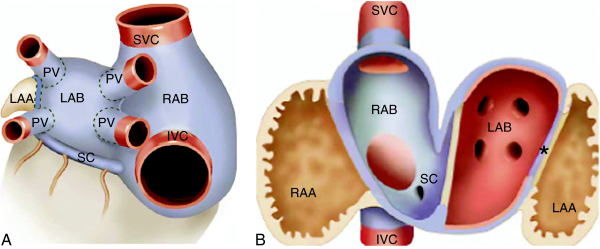
\includegraphics[scale=4.0]{PVatriumTissue.png}
\caption{Schematic depiction of outer side of atrial chambers with pulmonary veins (PV), left atrial appendage (LAA), left atrial body (LAB), right atrial body (RAB), superior vena cava (SCV) and inferior vena cava (IVC). LAB and RAB are covered by myocardium (heart muscle tissue) with smooth-walled inner aspect (blue), which streches out over extracardiac segments of PV (blue area above and below dotted line). Figure taken from \cite{Dou06}}
\end{center}
\end{figure}

Recent studies have shown that \textbf{rotors} might be another possible trigger for AF. Animal and computer models indicate that anisotropic re-entries may perpetuate AF \cite{Jal03}. A periodic activity of a small number of rotors in the posterior left atrial wall PV region may activate the atria at exceedingly high frequencies and result in AF.\newline

Furthermore, according to the \textbf{multiple wavelet hypothesis} AF is sustained by the continous propagation of  several independent wavelets \cite{CE09}. These wavelets are propagating through the muscles of the atria in a chaotic manner. Interference effects between various wavelets lead to amplification or cancellation. As long as the number of wavefronts does not decline a certain threshold level AF is sustained.\newline

Certain risk factors and indicators for AF can be found in the AF patient group \cite{CE09}. Ageing generally increases the risk of developing AF. The reason might be due to age dependent loss of atrial myocardium and the associated conduction disturbances. Hypertension is also an age dependent factor which is a risk factor for the incidence of AF as well as AF-related complications such as stroke and systematic thromboembolism. These complications are most likely also induced by the possible alterations in the heart due to AF. Atrial contraction is modified, ventricular rates usually increased and become irregular. Furthermore abnormalities in the blood flow are evident resulting e.g. in reduced left atrial appendage flow velocities, in an area which is considered the main site of thrombus formation in AF patients \cite{ESC12}. Thyroid dysfunction can be the sole cause of AF and may induce AF related complications. 25 \% of AF patients are obese \cite{Nab09} and 20 \% suffer of diabetes mellitus requiring 
medication. Chronic obstructive pulmonary disease (COPD) is found in 10 - 15 \% of AF patients. 
Nevertheless it is possibly more a marker of general cardiovascular risk then an indicator for AF. Chronic renal disease is present in 10 - 15 \% of AF patients and it is suggested that renal failure may increase the risk of AF related complications \cite{CE09}. Independent of the stated risk factors AF has also a genetic component, especially considering an early onset of AF. In a study carried out by Fox et al. \cite{Fox04} with 2243 offspring participants it was stated that the risk of developing AF compared to no parental AF was significantly increased (multivariable-adjusted odds ratio of 1.85, 95 \% confidence interval). The results were even stronger when age was limited to an age younger than 75 (multivariable-adjusted odds ratio of 3.23, 95 \% confidence interval). 


\subsection*{Treatment modalities}

The treatment modalities for AF have three main goals: to reset the rhythm, to control the rate and to prevent the formation of blood clots \cite{Mayo} \cite{CE09}. The treatment strategie chosen for each individual patient depends on the type of AF and on careful consideration of patient individual factors, including potential further heart problems. \newline

Resetting the heart rhythm is carried out by cardioversion, either based on medication (anti-arrhythmic drugs) or electrically. In an electrical cardioversion an electrical shock is delivered to the heart of a sedated patient via paddles or patches. The shock stops the heart for a moment, giving the conduction system of the heart the possibilty to restore its normal activity. Commonly used anti-arrhythmic drugs are e.g. Amiodarone and Dronedarone. These drugs have severe side effects and can act proarrhythmic, causing also 
life-threatening ventricular arrhythmias \cite{Mayo}. Furthermore the risk of another AF episode is not reduced.\newline

Once AF can be converted to a normal heart rhythm, the heart rate needs to be reduced to a normal pace between 60 and 100 beats per minute. Heart rate control can be achieved either by the usage of different medication or by AV node ablation. Medications include for example Lanoxib, which can control the heart rate at rest but not during physical activity so that additional medication like calcium blockers or beta blockers are needed. In case that the medication is not working or the side effects are to severe AV node ablation is carried out as alternative treatment modality. Via a catheter the AV node is ablated, blocking the signals coming from the atria passing to the ventricles. This procedure requires simultaneoulsy the implamentation of a pacemaker to establish a heart beat. With this procedure the atria is still fibrillating, so that further medication with anti-arrhythmic medication as well as anticoagulants is required.\newline

For paroxysmal or persistent AF alternative treatment modalities include radiofrequency catheter ablation or the surgical maze procedure.\newline
The maze procedure is carried out during an open heart surgery and hence allows for very precise lesion patterns. Scar tissue in the atria is 
created by either using a scalpel, radiofrequency energy or cryotherapy. The procedure has a very good success rates. In a recently published 
analysis of 48 studies (involving 3832 patients) it resulted that sinus rhytm was maintained in 83 \% of patients who underwent 
the maze procedure \cite{CE09} \cite{Kha05}. Nevertheless it requires open heart surgery, making it unsuitable for many patients. It is thus 
generally reserved to patients who do not respond to other treatment modalities or if it can be combined with other procedures which require 
heart surgery. \newline
In catheter ablation the main strategie is anatomic based, which means that it is assumed that AF is triggered and sustained by the same 
antomical sites (the PVs) in the majority of AF patients \cite{CE09}. In radiofrequency ablation a catheter is inserted into the patient 
through an arteria close to the groin of the patient and fed to heart. The energy is then used to make areas close to the junction between 
the pulmonary veins and the atria desolate.\newline

Various ablation techniques exist, including the PV isolation by 
segmental ostial ablation, circumferential PV ablation, wide-area circumferential ablation and antral PV isolation \cite{Ora06} \cite{Ora03} 
\cite{Ouy04}. Antral PV isolation and wide-area circumferential ablation was shown to be effective for both patients with paroxysmal and 
persistent AF \cite{CE09} \cite{Ora03}. In a randomized study circumferential PV ablation was found to result in a sinus rhythm in 74 \% of 
patients with chronic AF \cite{Ora06}. Linear ablation is another ablation technique which is either performed in combination with PV 
isolation or circumferential ablation or as stand alone technique \cite{CE09}. The motivation for this procedure is to interrupt reentries.

%%%% FIGURE: ABLATION

Endpoints during PV isolation is to induce a complete electrical isolation of the PVs. This is confirmed by elimination of all PV potentials 
as well as entrance and exit block during pacing at multiple sites within the PVs \cite{CE09}. Freedom from recurrent AF can be predicted 
by termination and noninducibility of AF during catheter ablation \cite{} \cite{} \cite{} \cite{}. Termination of AF indicates elimination 
of all triggers and drivers of AF while noninducibility indicates the absence of residual trggers and drivers that may initiate and 
perpetuate AF \cite{CE09}. Termination is hence not a reliable predictor in patients with paroxysmal AF while noninducibility is likely 
to predict that the patients are going to stay in sinus rhythm. 

%%%% FIGURE: PREDICTION AF

% Alternatively also ablation with cryotherapy can be carried out, in which the heart tissue is not made desolate but rather freezed.\newline



Independent of the used procedure, anticoagulants like Warfarin are used in a diversity of patients. In order to establish international criterias for risk patients who should uptake anticoagulants, the CHADS$_{2}$-VASc score was defined \cite{ESC12}.

\begin{itemize}
 \item [] \textbf{C}ongestive heart failure: 1 point
 \item [] \textbf{H}ypertension: 1 point
 \item [] \textbf{A}ge ($\geq$ 75): 2 points
 \item [] \textbf{D}iabetes mellitus: 1 point
 \item [] \textbf{S}troke: 2 points
 \item [] \textbf{V}ascular disease: 1 point
 \item [] \textbf{A}ge (65-74): 1 point
 \item [] \textbf{S}ex (female): 1 point
\end{itemize}

Patients who obtain at least 2 point in the CHADS$_{2}$-VASc score are prescribed anticoagulants. Patients with 1 point might be prescribed anticoagulants, alternatively asprin can be used. Patients with a score of 0 are supposed to only take asprin \cite{Fle}. The CHADS$_{2}$-VASc score has been validated in multiple cohorts \cite{Lip11} and it was shown that the CHADS$_{2}$-VASc is better then other scores (like the CHADS$_{2}$ score) at identifying low risk patients \cite{Pot12} \cite{Ole12} \cite{Van11} and as good as (or possibly better then) other scores in identifying patients who will develop strokes and thromboembolism \cite{Fri12} \cite{Ole11} \cite{Bor11}. 



\subsubsection*{Catheter ablation of AF: success rate and complications}

The FAST trial compared the outcome of catheter ablation and surgical ablation in a randomized study with a small patient population. 
The complication rate in surgical ablation was significantly higher but at the same time the success rate in treatment outcome was reduced 
in catheter ablation \cite{Boe12}. \newline

In two so-far conducted, nationwide survey the success rates of catheter ablation as a treatment 
for AF was studied. The first worldwide, multicenter survey was published in 2005 using data from 181 centers from 1995 to 2002. 
As a conclusion of this survey it was stated that 52 \% of AF patients undergoing ablation were symptom free without the need of further 
antiarrhythmic medication, 23.9 \% with the need of antiarrhythmic drugs. For the remaining patients a successful treatment outcome required 
a second (24.3 \%) or third (3.1 \%) procedure \cite{Cap05}. In the second worldwide, multicenter survey, which was performed inbetween 2003 
and 2006, an improvement in treatment outcome was shown. The rate for a successful treatment outcome without the need of further antiarrhythmic 
medication increased to 70 \% while the rate with the need of further antiarrhythmic medication decreased to 10 \%, resulting in an overall 
success rate of 80 \% compared to 75.5 \% in the first survey. The second study did not indicate any information on the percentage of patients 
needing more than one procedure. When broken down by type of AF, the success rate without antiarrhythmic drugs was 75\% for paroxysmal AF, 
65\% for persistent AF, and 63\% for longstanding persistent AF \cite{Cap10} \cite{Sto}.\newline

The complication rates were studied in an European survey from 2012 \cite{Arb12}. The acute severe complication rates of over 1000 ablation 
procedures carried out high-volume centers throughout Europe were reported to be 0.6 \% for stroke, 1.3 \% for tamponade, 1.3 \% for 
peripheral vascular complications and 2 \% for pericarditis. Similar numbers were reported in an US study \cite{Hoy11} \cite{Cap10}. 
These informations were obtained from voluntary survey responses and are thus likely to be biased, making the true complications rate 
higher than stated. In a recent analysis in 4156 patients who had an ablation procedure between 2005 and 2008 it was stated that the 
complication rate was 5 \% and that the rate of hospitalization in the first year after ablation was 38.5 \% (including all possible causes) 
\cite{Sha12}. Ongoing trials are expected to give more insights in the next years. For now, risk associated with AF ablation needs to be carefully 
weighed against individual symptomatic benefit \cite{ESC12}. 



\begin{thebibliography}{9999999}
 \bibitem[amc]{amc}{Arthur's Medical Clipart, arthursclipart.org}
 \bibitem[afib]{afib}{Atrial fibrillation Resources for patients, a-fib.com}
 \bibitem[Arb12]{Arb12}{Arbelo E, Brugada J, Hindricks G, Maggioni A, Tavazzi L, Vardas P, Anselme F, Inama G, Jais P, Kalarus Z, Kautzner J, Lewalter T, Mairesse G, Perez-Villacastin J, Riahi S, Taborsky M, Theodorakis G, Trines S; on behalf of the Atrial Fibrillation Ablation Pilot Study Investigators. ESC-EURObservational research programme: the atrial fibrillation ablation pilot study, conducted by the European Heart Rhythm Association. Europace 2012;14:1094 –1103}
 \bibitem[Boe12]{Boe12}{Boersma LV et al: Atrial fibrillation catheter ablation vs. surgical ablation treatment (FAST): a 2-center randomized clinical trial; Circulation 125; 23-30; 2005}
 \bibitem[Bor11]{Bor11}{Boriani G et al: Italian AT-500 Registry Investigators. Improving stroke risk stratification using the CHADS$_{2}$ and CHADS$_{2}$-VASc risk score in patients with paroxysmal atrial fibrillation by continous arrhythmia burden monitoring; Stroke 42; 1768-1770; 2011}
 \bibitem[Cap05]{Cap05}{Cappato R et al: Worldwide Survey on the Methods, Efficacy, and Safety of Catheter Ablation for Human Atrial Fibrillation; Circulation 111; 1100-1105; 2005}
 \bibitem[Cap10]{Cap10}{Cappato R, Calkins H, Chen SA, Davies W, Iesaka Y, Kalman J, Kim YH, Klein G, Natale A, Packer D, Skanes A, Ambrogi F, Biganzoli E: Updated Worldwide Survey on the Methods, Efficacy, and Safety of Catheter Ablation for Human Atrial Fibrillation; Circulation: Arrhythmia and Electrophysiology 3; 32-38; 2010} 
 \bibitem[CE09]{CE09}{Cardiac Electrophysiology: From Cell to Bedside, Zipes and Jalife, Saunders Elsevier, 5th Edition, 2009}
 \bibitem[Dou06]{Dou06}{Douglas YL, Jongbloed MR, Gittenbergerde Groot AC et al: Histology of vascular myocardial wall of left atrial body after pulmonary venous incorporation; Am J Cardiol 97; 662-670; 2006}
 \bibitem[ESC10]{ESC10}{ESC Guidlines for the management of atrial fibrillation: The task force for the Management of Atrial Fibrillation of the European Society of Cardiology (ESC); European Heart Journal 31; 2369-2429; 2010}
 \bibitem[ESC12]{ESC12}{2012 focused update of the ESC Guidlines for the management of atrial fibrillation: An update of the 2010 ESC Guidlines for the management of atrial fibrillation; European Heart Journal; 2012}
 \bibitem[Fle]{Fle}{http://flexikon.doccheck.com/de/CHA2DS2-VASc-Score}
 \bibitem[Fox09]{Fox09}{Fox CS et al: Parental atrial fibrillation as a risk factor for atrial fibrillation in offspring; JAMA 291; 2851-2855; 2004}
 \bibitem[Fri12]{Fri12}{Friberg L et al: Evaluation of risk stratification schemes for ischaemic stroke and bleeding in 182 678 patients with atrial fibrillation: the Swedish Atrial Fibrillation Cohort study; Eur Heart J 33; 1500-1510; 2012}
 \bibitem[Hai98]{Hai98} {Ha\"{\i}ssagurre M, Jais P, Shah DC et al: Spontaneous initiation of atrial fibrillation by etopic beats originating in the pulmonary veins; N Engl J Med 339; 659-666; 1998}
 \bibitem[Hoy11]{Hoy11}{Hoyt H, Bhonsale A, Chilukuri K, Alhumaid F, Needleman M, Edwards D, Govil A, Nazarian S, Cheng A, Henrikson CA, Sinha S, Marine JE, Berger R, Calkins H, Spragg DD. Complications arising from catheter ablation of atrial fibrillation: temporal trends and predictors. Heart Rhythm 2011;8:1869 – 1874.}
 \bibitem[Jal03]{Jal03}{Jalife J: Rotors and spiral waves in atrial fibrillation; J Cardiovasc Electrophysiol 14; 776-780; 2003}
 \bibitem[Kha05]{Kha05}{Khargi K, Hutten BA, Lemke B, et al: Surgical treatment of atrial fibrillation; a systematic review; Eur J Cardiothorac Surg 27; 258-265; 2005}
 \bibitem[Lip11]{Lip11}{Lip GY: Stroke in atrial atrial fibrillation: epidemiology and thromboprophylaxis; J Thromb Hearnost 107; 1053-1065; 2011}
 \bibitem[Mayo]{Mayo}{Atrial fibrillation: Health information, mayoclinic.com}
 \bibitem[Med]{Med}{XXXX}
 \bibitem[Miy06]{Miy06}{Miyasak Y, Barnes ME, Gersh BJ et al: Secular trends in incidences of atrial fibrillation in Olmsted County, Minnesota, 1980 to 2000, and implications on the projection for future prevalence; Circulation 115; 119-125, 2006}
 \bibitem[Nab09]{Nab09}{Nabauer M et al: The registry og the German Competence Network on atrial fibrillation: patient characteristics and initial management; Eurospace 11; 423-434; 2009}
 \bibitem[Ole11]{Ole11}{Olesen JB et al: Validation of the risk stratification schemes for predicting stroke and thromboembolism in patients with atrial fibrillation: nationwide cohort study; Br Med J 342; 2011}
 \bibitem[Ole12]{Ole12}{Olesen JB et al: The value of the CHADS$_{2}$-VASc score for refining stroke risk stratification in patients with atrial fibrillation with a CHADS$_{2}$ score 0-1: a nationwide cohort study; Thromb Haernost 107; 1172-1179; 2012}
 \bibitem[Ora03]{Ora03}{Oral H, Scharf C, Chugh A, et al: Catheter ablation for paroxysmal atrial fibrillation: Segmental pulmonary vein ostial ablation versus left atrial ablation; Circulation 108; 2355-2360; 2003}
 \bibitem[Ora06]{Ora06}{Oral H, Pappone C, Chugh A, et al: Circumferential pulmonary-vein ablation for chronic atrial fibrillation; N Engl J Med 354; 934-941; 2006}
 \bibitem[Ouy04]{Ouy04}{Ouyang D, Bansch D, Ernst S, et al: Complete isolation of left atrium surrunding the pulmonary veins: New insights from the double-Lasso technique in paroxysmal atrial fibrillation; Circulation 110; 2090-2096; 2004}
 \bibitem[Pot12]{Pot12}{Potpara TS et al: Reliable identification of 'truly low' thromboembolic risk in patients initially initially diagnosed with 'lone' atrial fibrillation: the Belgrade Atrial Fibrillation Study; Circ Arrhythm Electrophysiol 5; 319-326; 2012}
 \bibitem[Sha12]{Sha12}{Shah RU, Freeman JV, Shilane D, Wang PJ, Go AS, Hlatky MA. Procedural complications, rehospitalizations, and repeat procedures after catheter ablation for atrial fibrillation. J Am Coll Cardiol 2012;59:143 –149}
 \bibitem[Sto]{Sto}{http://www.stopafib.org/catheter-ablation/success-rates.cfm}
 \bibitem[Van11]{Van11}{Van Staa TP et al: A comparison of risk stratification schemes for stroke in 79,884 atrial fibrillation patients in general pratice; J Thromb Haernost 9; 39-48; 2011}

 \end{thebibliography}




\end{document}